\chapter{Coding the Models}\label{chap:codingTheModels}

\section{Programming Languages}

One of the first considerations when performing any machine learning task is often deciding which language should be used for building the model and performing inference. Engineers often use MATLAB for their calculations, but its features are not suitable for these purposes.

\subsection{Object Oriented Languages}

Object oriented programming is based on the concept of defining ``objects", which are instances of classes and have properties, and associated procedures or ``methods". Some key features of object oriented languages are:

\begin{itemize}

\item \textbf{Encapsulation:} information hiding - only authorised parties may access data. This helps to avoid unwanted side-effects and allows type-checking on method calls.
\item \textbf{Inheritance:} the ability to create class hierarchies with classes inheriting features from their parent
\item \textbf{Polymorphism:} subclasses may inherit methods but change their functionality

\end{itemize}

Object oriented programming is modular, allowing separation of code into different modules. This encourages extensibility and code re-use. It also allows updates to be made more easily without requiring large-scale changes. Programs are typically quicker to build and more cost effective.

\subsubsection{Java}

Java is an object oriented language created by Sun Microsystems. It has the tagline ``write once, run anywhere", meaning that the code does not need to be recompiled to run on a new system architecture. Applications are compiled to byte code and can run on any Java Virtual Machine (JVM).

Some key benefits of using Java are:

\begin{itemize}

\item It is free
\item There is a large standard class library
\item There is comprehensive documentation available 

\end{itemize}

Java has been used in the past to create a version of the Sequence Memoizer. However...

\todo[inline]{Discussion of Java}


\subsubsection{C++}

C++ is another object oriented language in which the Sequence Memoizer has already been implemented. It has been around for much longer than Java and is based on another language, C. Although there is a large amount of support available, it is generally considered to be a more difficult language to learn than Java.

\todo[inline]{Discussion of C++}

\subsection{Functional Languages}

Functional languages execute programs by evaluating expressions. Functions can be passed to other functions as arguments or returned as the result of a function. They typically have immutable data, i.e. instead of altering values, variables are instead copied and then altered. Another key feature is that of ``lazy" evaluation. Lazy expressions are evaluated only when their result is required. This allows for the definition of infinite data structures. Recursion is commonly used in functional programming. 

%\subsubsection{Scala}
%
%Scala is a functional language that runs on the JVM. It retains many of the features of object oriented languages in the sense that every value is an object. It also interoperates with Java and can make use of the wide codebase available.
%
%\todo[inline]{More info on Scala}

\subsubsection{Lisps}

Lisp is a family of functional languages with parenthesised syntax. The name derives from ``LISt Processing", as linked lists are one of the major data structures used. Function calls are written as a parenthesised list with the function name as the first element, followed by any arguments. For example, \lstinline!(func arg1 arg2)!. This syntax makes it very easy to nest function calls. Lisps also have a strong reliance on recursion, making them ideal for the purposes of this project. 

Macros are a very important feature of Lisps. These are similar to functions, but generally generate code to be compiled and executed. This happens before runtime and allows the developer to add new features to the code.



\subsection{Language Choice}

The final choice of language for implementing the models was Clojure. Clojure is a Lisp language that runs on the JVM. Its compact syntax makes coding the complex functions and data structure relatively simple. There are also many  built-in functions that are particularly useful for this project's purposes, for example, \lstinline!frequencies!, which counts the number of occurrences of each unique value in a sequence, or \lstinline!first! and \lstinline!last!, which allow for easy selection of the first and last entries in a set.

Clojure allows the use of \textit{memoization}, which greatly increases processing speeds. This is the technique of storing already calculated results in cache so that they need not be computed again if a function is called with the same arguments. Throughout this project, all functions were memoized where possible.

Clojure has its own built-in ``terminal" called the \textit{REPL}. This stands for ``Read-Eval-Print Loop". The REPL makes experimenting with code very easy, as the user can input commands and write code ``on the fly" without needing to edit the source code and re-launch the program.



\section{Integrated Development Environment}

Eclipse is a freely available \textit{Integrated Development Environment} (IDE), an application with facilities for software development. It is mainly intended for use with Java, but a plugin called Counterclockwise exists for Clojure development. Since it is an IDE with which I was already familiar, it seemed a logical choice for this project. 

\section{Version Control}

GitHub is an online hosting service for projects using Git \textit{version control}, a way of managing changes to files. Git records any changes made to tracked files and keeps a record of these. This means that changes can be reversed at any time and it is possible to revert to a previous version of the code. For collaborative projects, this makes it easy for multiple users to edit different parts of the code. 

An online GitHub account links to a Git repository, where the code is stored. Members of a team can then ``pull" the latest version of this code to their local filesystem. After editing a file, the user can then ``push" their changes back to the repository so that all other users can have the latest updates. 

\section{Program Architecture}

The Clojure code was divided into \textit{packages} (like modules) and \textit{namespaces} (like classes). The \textit{core} file (like the \textit{main} method in Java programs) contains the first code executed at run time. All other namespaces are employed using the \lstinline!require! keyword. 

The namespace hierarchy for this project is detailed in Figure \ref{fig:namespaceHierarchy}.

\begin{figure}[h]
\centering
\begin{tikzpicture}
\node{\Tree[.$\bullet$ core [.\textit{letters} file\_reader hierarchical\_dirichlet letter\_maker letter\_predictor letter\_probs ] [.\textit{words} file\_reader good\_turing interpolation word\_maker word\_predictor word\_probs ] [.\textit{misc} misc\_functions ] ]};
\end{tikzpicture}
\caption{Code Architecture}
\label{fig:namespaceHierarchy}
\end{figure}

\todo[inline]{Architecture Diagram}
